\ctitle{Cellebiologi}

\paragraph{Dette kapittelet} er en innføring i hvordan celler er bygget opp, samt litt om hvordan celler tar opp og bruker energi (metabolisme).

\cstitle{Celler}
\paragraph{Celle}\index{celle} Den fundamentale enheten for liv. 

\noindent Alle celler
\begin{itemize}[nolistsep,noitemsep]
	\item er avgrenset fra omgivelsene med en cellemembran,
	\item er åpne systemer med metabolisme (de tar opp næringsstoffer fra miljøet, transformerer dem, og slipper ut avfallsstoffer i miljøet),
	\item er i stand til å vokse ved å omforme kjemikaler fra miljøet til nye celler, og
	\item inneholder gener, og er del av en evolusjonsprosess: endringer i genene videreføres til etterkommere.
\end{itemize}

\noindent Noen celler
\begin{itemize}[nolistsep,noitemsep]
	\item kan bevege seg på egenhånd ved hjelp av spesialiserte strukturer (dette kalles \idx{motilitet}),
	\item kan forandre form og egenskaper i løpet av forskjellige faser i en livssyklus (dette kalles \idx{differensiering}),
	\item kan kommunisere og interagere med andre celler ved hjelp av kjemikalier som tas opp og slippes løs i miljøet, eller
	\item kan overføre arvematerialer til og fra andre celler (dette kalles \idx{horisontal genetisk utveksling}).
\end{itemize}

\paragraph{Katalytiske funksjoner}\index{katalytiske funksjoner} Celler utfører kjemiske reaksjoner som akselereres via enzymer. Dette beskrives i Kapittel 2. De katalytiske funksjonene til en celle fasiliterer cellevekst, og inkluderer lagring av energi i form av ATP, samt dannelse av forløperne til makromolekyler som karbohydrater, aminosyrer og fettsyrer.

\paragraph{Genetiske funksjoner}\index{genetiske funksjoner} Celler lagrer og prosesserer genetisk informasjon, som videreføres til etterkommere gjennom reproduksjon. Denne informasjonen er lagret som DNA. De genetiske funksjonene til en celle fasiliterer reproduksjon. Genetiske funksjoner i cellen inkluderer transkripsjon (produksjon av RNA fra DNA) og translasjon (produksjon av proteiner fra RNA).

\paragraph{Prokaryot celle}\index{prokaryot} En kategori relativt enkle celler som omfatter \ix{bakterier} og \ix{arkebakterier}. Navnet kommer fra det greske \emph{karyon} (kjerne), og forteller at dette er cellene som fantes før (\emph{pro}) det fantes organismer med cellekjerne. Det hender at ``bakterie'' og ``prokaryot'' brukes om hverandre litt upresist, men det går stort sett fint.

\noindent Alle prokaryoter har
\begin{itemize}[nolistsep,noitemsep]
	\item en \idx{cytoplasmamembran} (se eget avsnitt),
	\item en \idx{nukleoid}: sirkulært DNA som inneholder den genetiske koden til organismen, som \emph{ikke} ligger i en cellekjerne, og
	\item \idx{ribosom}er, som utfører translasjon (lager proteiner fra RNA). 
\end{itemize}
\noindent De fleste prokaryoter har
\begin{itemize}[nolistsep,noitemsep]
	\item \idx{plasmid}er: små, ekstra fragmenter av DNA utenfor nukleoiden,
	\item en \idx{cellevegg} som beskytter cellen mekanisk og kjemisk fra omgivelsene og er et ekstra beskyttende lag, og/eller
	\item \idx{flagella og pili} (strukturer på utsiden av cellen som gjør cellen i stand til å bevege seg på egenhånd og kommunisere med andre celler).
\end{itemize}

\paragraph{Eukaryot celle} Cellene som planter, dyr og sopper består av. De er større og mer komplekse enn prokaryote celler. De har forskjellige kompartementer som utfører spesifikke metabolske oppgaver og er adskilt fra hverandre med membraner.

\noindent Alle eukaryoter har
\begin{itemize}[nolistsep,noitemsep]
	\item en \idx{cellekjerne}, som inneholder cellens DNA, organisert i form av kromosomer,
	\item \idx{mitokondrier} som genererer energi,
	\item en cytoplasmamembran (se under),
	\item ribosomer,
	\item \idx{endoplasmatisk retikulum}, et transportnettverk for molekyler som skal til bestemte steder, og
	\item et \idx{golgiapparat} som prosesserer og pakker makromolekyler som syntetiseres av cellen, f.eks proteiner og lipider.
\end{itemize}
\noindent Noen eukaryoter har
\begin{itemize}[nolistsep,noitemsep]
	\item \idx{kloroplaster}, også kjent som grønnkorn, som utfører fotosyntese, og
	\item cellevegg.
\end{itemize}

\paragraph{Cellemorfologi}\index{cellemorfologi} Morfologi er læren om form, og celler kan ha forskjellige former. De vanligste celleformene for prokaryoter er coccus (kulerunde eller eggformede), stav (sylindriske) og spirillum (spiralformede). Faktorer som kan påvirke cellemorfologi er
\begin{itemize}[nolistsep,noitemsep]
	\item Optimalisering av næringsopptak. Dette favoriserer små celler med stort areal per volum, siden næringsopptak skjer ved celleoverflaten.
	\item Svømmeevne i tyktflytende medier eller nær overflater. Dette favoriserer spiralformede celler.
	\item Glideevne. Dette favoriserer tynne bakterier.
\end{itemize}

\paragraph{Cytoplasmamembran}\index{cytoplasmamembran} Halvgjennomtrengelig membran som omringer cellen, og skiller innholdet i cellen (cytoplasmaet) fra miljøet. Den er 6-8nm tykk. Den består av et dobbeltlag av \ix{fosfolipider} der de hydrofobe karbonkjedene er vendt mot hverandre og de hydrofile fosfat/glyserol-endene er vendt utover mot miljøet og innover mot cytoplasmaet. Det finnes andre variasjoner over samme tema, der andre kjemiske grupper er bundet til glyserol-``ryggraden''. 

\paragraph{Proteiner i cytoplasmamembranen} Det finnes proteiner som ``setter seg fast'' inne i cellemembranen. Disse kalles \idx{membranproteiner}. De kan enten stikke ut på en side (perifere membranproteiner) eller på begge (dvs. at de går tvers igjennom - integrale membranproteiner). Dette stabiliseres av hydrogenbindinger. I tillegg kan \ce{Mg^2+} og \ce{Ca^2+}-ioner stabilisere membranen ved å lage ionebindinger.

\paragraph{Membranforsterkere} Noen membranforsterkende stoffer er \idx{steroler} (stive plane lipider som finnes i eukaryoter) og \idx{hopanoider} (ligner på steroler og finnes i bakterier).

\paragraph{Funksjonene til cytoplasmamembranen} Cytoplasmamembranen
\begin{itemize}[nolistsep,noitemsep]
	\item er en halvtgjennomtrengelig membran som er spesifikk nok til at næringsstoffer kommer inn og avfallsstoffer går ut (ved hjelp av transportproteiner), selv om konsentrasjonsgradienten i miljøet skulle tilsi det motsatte,
	\item er et anker for viktige proteiner (som beskrevet over), og
	\item spiller en viss rolle i energilagring: det produseres eller brukes energi når ioner passerer cellemembranen, avhengig av om ionet henholdsvis følger konsentrasjonsgradienten eller går motsatt vei av den.
\end{itemize}

\paragraph{Regler for bevegelse gjennom cellemembranen}
\begin{itemize}[nolistsep,noitemsep]
	\item Enkelte små uladde molekyler (som vann) kan passere gjennom \ix{passiv diffusjon}.
	\item Store molekyler og små ladde molekyler kan ikke passere gjennom membranen på passivt vis, men må delvis degraderes før opptak. For eksempel må proteiner degraderes til aminosyrene de består av.
	\item Mange typer molekyler kan passere gjennom aktive transportsystemer - disse prosessene er forskjellige fra stoff til stoff, og kan kreve energi ved bruk av ATP.
\end{itemize}

\cstitle{Metabolisme}
\paragraph{Metabolisme}\index{metabolisme} De livgivende kjemiske reaksjonene som foregår i celler. Den deles opp i katabolisme og anabolisme.

\paragraph{Katabolisme}\index{katabolisme} Den delen av metabolismen som bryter ned organiske stoffer til enklere stoffer og henter energi gjennom en rekke kjemiske reaksjoner som kalles \idx{celleånding}. Alle avsnittene mellom dette og ``Anabolisme'' omhandler aspekter ved katabolisme.

\paragraph{Metabolsk diversitet}\index{metabolsk diversitet} Forskjellige mikroorganismer har gjennom 4 milliarder år med evolusjon utviklet metoder for å oppta energi fra miljøet på nesten alle tenkelige måter. Figur \ref{fig:metabolicdiversity} viser en oversikt over metabolsk diversitet: organismer som bruker lys som energikilde kalles \idx{fototroper} - dette kan skje ved \idx{oksygenisk fotosyntese} (produserer oksygen) eller \idx{anoksygenisk fotosyntese} (produserer ikke oksygen). Andre organismer kalles \idx{kjemotrofer} og opptar energi ved å oksidere kjemisk drivstoff. Organismer som bruker uorganiske stoffer (\ce{H2, H2S, Fe^2+, NH4^+}, etc) som energikilde kalles \idx{kjemolitotrofer} - kun prokaryoter er kjemolitotrofer. Organismer som bruker organiske stoffer (glukose, acetat, etc.) som energikilde kalles \idx{kjemoorganotroper} - \idx{aerobe organismer} bruker oksygen for å ta opp energi og \idx{anaerobe organismer} opptar energi i fravær av oksygen). Uansett hvordan energien er tatt opp fra miljøet, lagres den som ATP. 

\paragraph{Autotrofer og heterotrofer} Alle organismer trenger karbon. \emph{Autotrofer} får karbonet sitt fra \ce{CO2}, og kalles ofte \ix{primærprodusenter}. \idx{Heterotrofer} trenger ett eller flere organiske molekyler som kilde for karbon, og får tak i dette enten ved å spise \ix{autotrofer} eller produkter som produseres av autotrofer, eller ved å spise andre heterotrofer.

\paragraph{Ekstremofile organismer} Organismer som overlever i ekstreme habitater der de har funnet sin egen nisje, for eksempel kokende varme kilder, breer, og vann med ekstremt høy saltkonsentrasjon eller pH. Teknikkene som \ix{ekstremofile organismer} bruker for å takle slike miljøer, kan være interessante å studere, bruke og forsøke å gjenskape.

\begin{figure}[H]
	\centering
	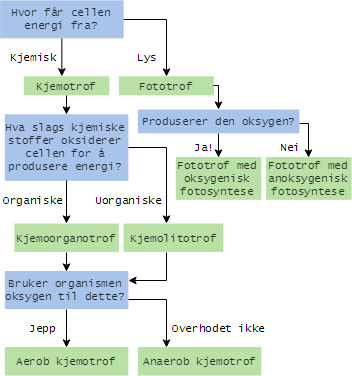
\includegraphics[width=0.45\textwidth]{metabolicdiversity}
	\caption{Klassifisering av organismer, basert på energikilde.}
	\label{fig:metabolicdiversity}
\end{figure}

\paragraph{Energibærere} Energivalutaen i celler er \emph{Adenosin trifosfat} (\ix{ATP}). ATP er det som produseres når cellen bryter ned næringsstoffer, og det som brukes når cellen skal gjøre noe som krever energi. Reaksjonen der ATP mister en fosfatgruppe for å bli adenosin difosfat (ADP) slipper løs 32 kJ/mol. De samme gjelder \ce{ADP -> AMP}. \ce{AMP ->}Adenosin slipper løs 14 kJ/mol når fosfat-adenosin-bindingen kuttes. Ett vannmolekyl inngår i hver slik spaltning.

\paragraph{Elektronbærere} Energibærere som overfører elektroner: nikotinamid adenin dinukleotid (\ix{NAD}) og flavin adenin dinukleotid (\ix{FAD}).

\paragraph{Langtidslagring av energi} Gjøres ved å lagre stoffer som uløselige polymerer som kan oksideres for å generere ATP. Noen eksempler er \ix{glykogen}, polyhydroksyalkanoater og svovel i prokaryoter; og stivelse og fettsyrer i eukaryoter.

\paragraph{Anabolisme} Den delen av metabolismen som lager cellens byggestoffer fra enklere stoffer gjennom energikrevende reaksjoner.

\paragraph{Cellens byggestoffer} er 
\begin{itemize}[nolistsep,noitemsep]
	\item karbohydrater (består av monosakkarider som glukose og fungerer som energilager samt en komponent i cellevegger),
	\item nukleinsyrer (består av nukleotider, brukes til å lagre, transportere og uttrykke genetisk informasjon),
	\item proteiner (består av aminosyrer, brukes til enzymer, som strukturelle komponenter og til transport av molekyler), og
	\item lipider (består av glyserol, fettsyrer og i noen tilfeller fosfat, fungerer som membraner (enten cytoplasmamembranen eller intracellulære kompartmenter)).
\end{itemize}

\paragraph{Aerob glukosemetabolisme} Aerob \ix{glukosemetabolisme} er cellens mest effektive metode for å produsere ATP. Det kalles også respirasjon, og involverer den vanlige reaksjonen for celleånding:
\begin{equation*}
	\ce{C6H12O6 + 6O2 ->[\text{38 ADP til ATP}] 6CO2 + 6H2O}
\end{equation*}

\paragraph{Anaerob glukosemetabolisme} Kalles fermentering, og involverer reaksjoner som 
\begin{equation*}
	\ce{C6H12O6 ->[\text{1-4 ADP til ATP}] 2C2H5O2 + 2CO2}
\end{equation*}
Det produseres mye mindre cellemasse gjennom fermentering enn ved respirasjon (kun 5\%). Reaksjonen krever mer glukose per ATP som blir produsert, og produserer sideprodukter som etanol. Eksempler på anaerob glukosemetabolisme er gjæring, og er når menneskekroppen danner melkesyre.

\paragraph{Gjæring} Når konsentrasjonen av \ce{O2} blir lav, endres genuttrykket i gjær slik at det er andre enzymer som aktiveres. I stedet for enzymene som utfører aerob metabolisme, aktiveres enzymene som utfører anaerob metabolisme. Dette er prinsippet bak gjøring.

\paragraph{Metabolsk spor} Et metabolsk spor er en tegning av veien fra næringsstoff til produkt, med piler mellom mellomprodukter. Skissering av metabolske spor med glukose som utgangspunkt sies å være veldig eksamensrelevant. 

\paragraph{Glukosemetabolisme} Figur \ref{fig:glucose} er en omformulering av figuren på slides, og kan med fordel pugges siden detaljer herfra har vært eksamensoppgaver. Det er naturligvis en del forenklinger her, blant annet forklares det ikke hvor man får vann fra. Man blir ikke så fryktelig klok på hvorfor glukosemetabolisme er relevant for resten av stoffet ved å se på denne figuren. Det blir man derimot ved å se på den utvidede figuren i Box 1.4 i Renneberg; når du er ferdig med å lese hele pensum kan du stirre lenge og vel på den figuren, og innse at nesten alle bioproduktene som har blitt diskutert til syvende og sist stammer fra nedbrytning av glukose.

\begin{figure}[H]
	\centering
	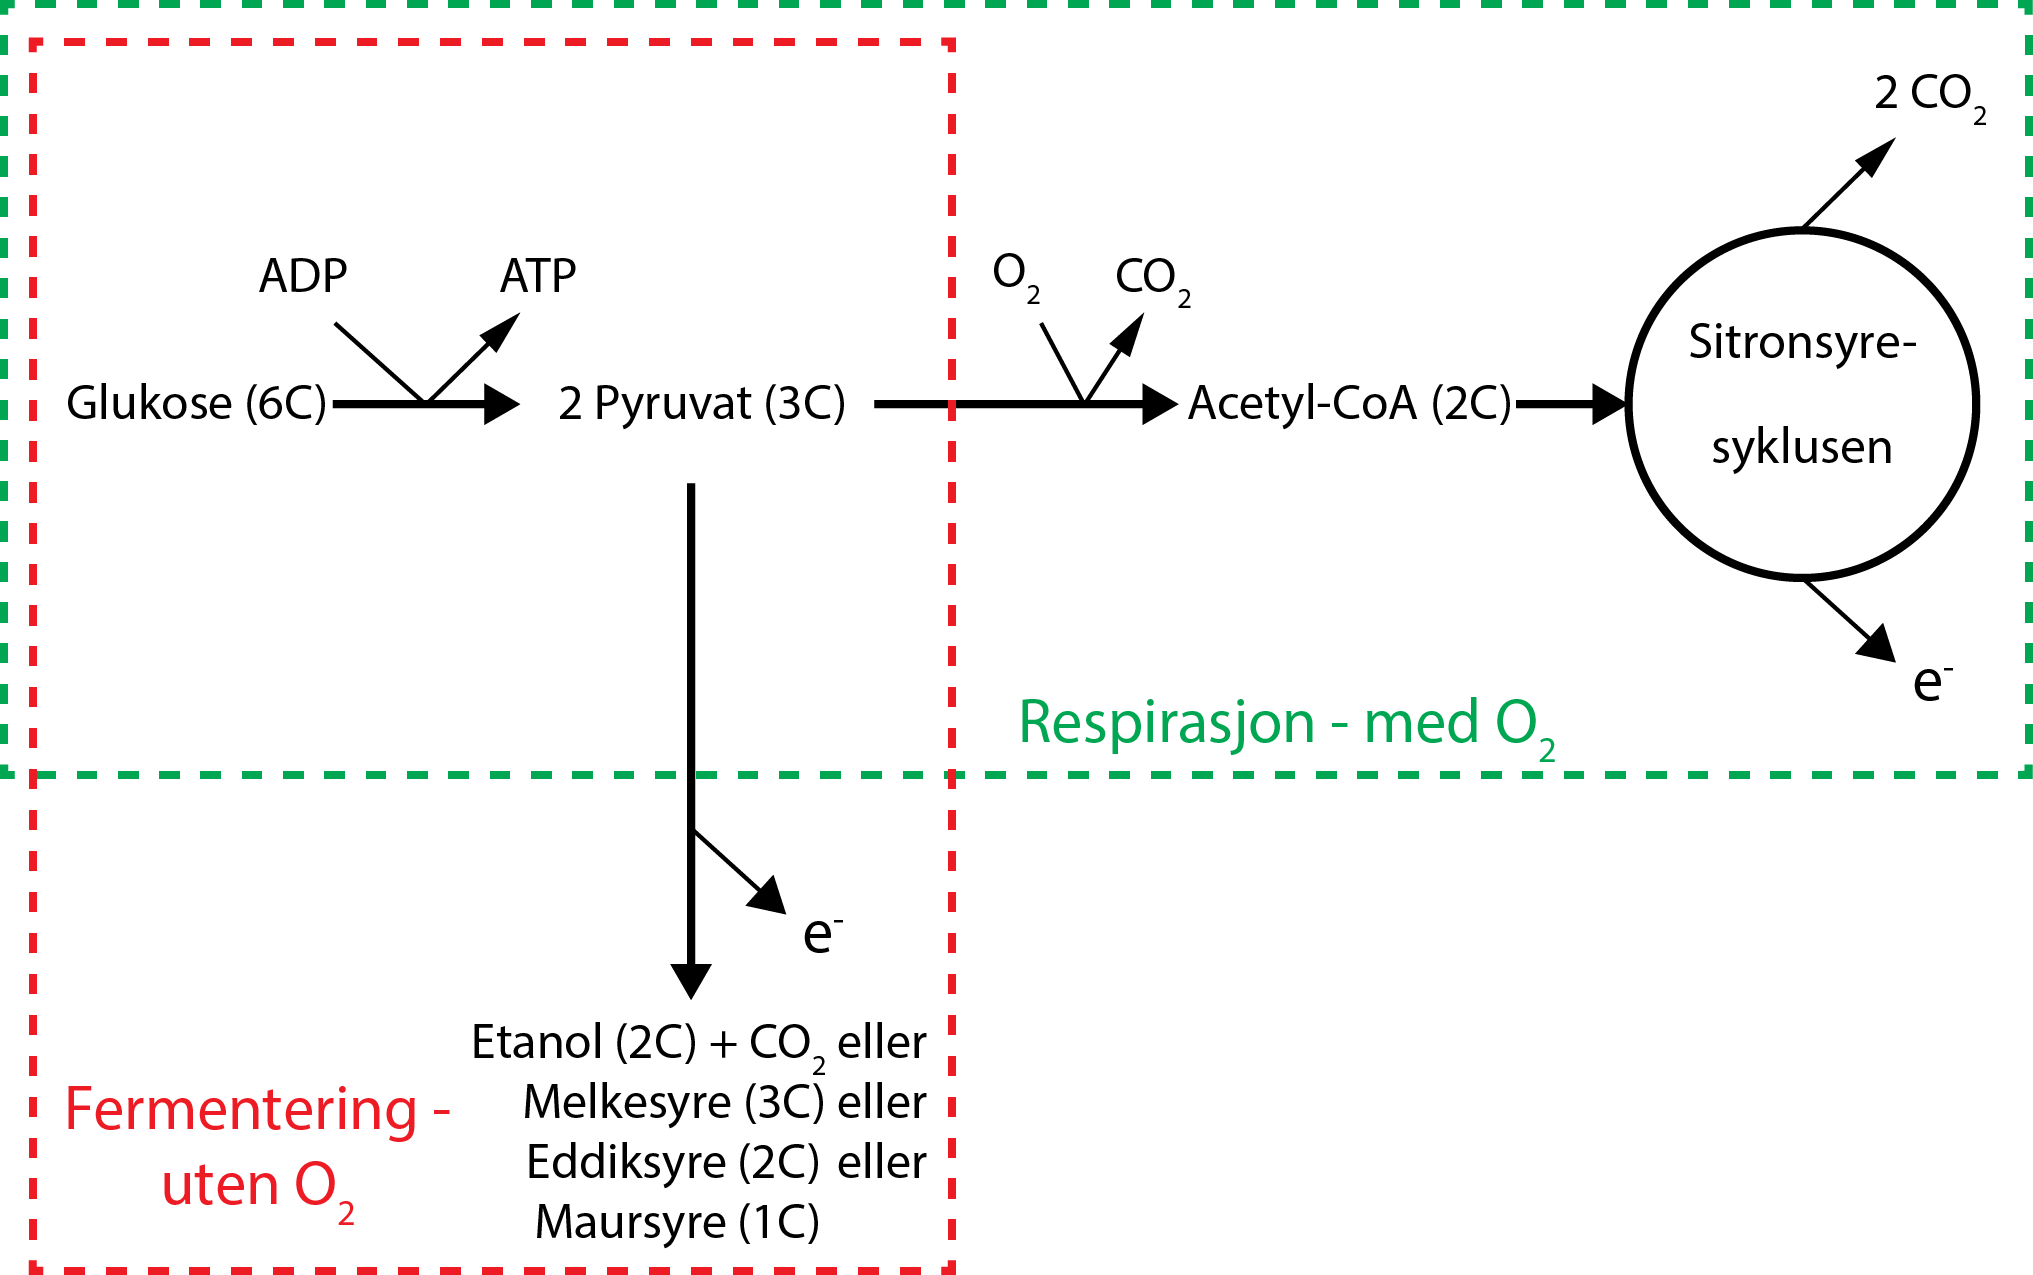
\includegraphics[width=0.45\textwidth]{glucose}
	\caption{Oversikt over glukosemetabolismen}
	\label{fig:glucose}
\end{figure}
